% Figure 5: spillover vs. corpus and model size. Drawn by dramatis scripts/paper_fig.py (make figures).
\begin{figure}[tbp]
  \centering
  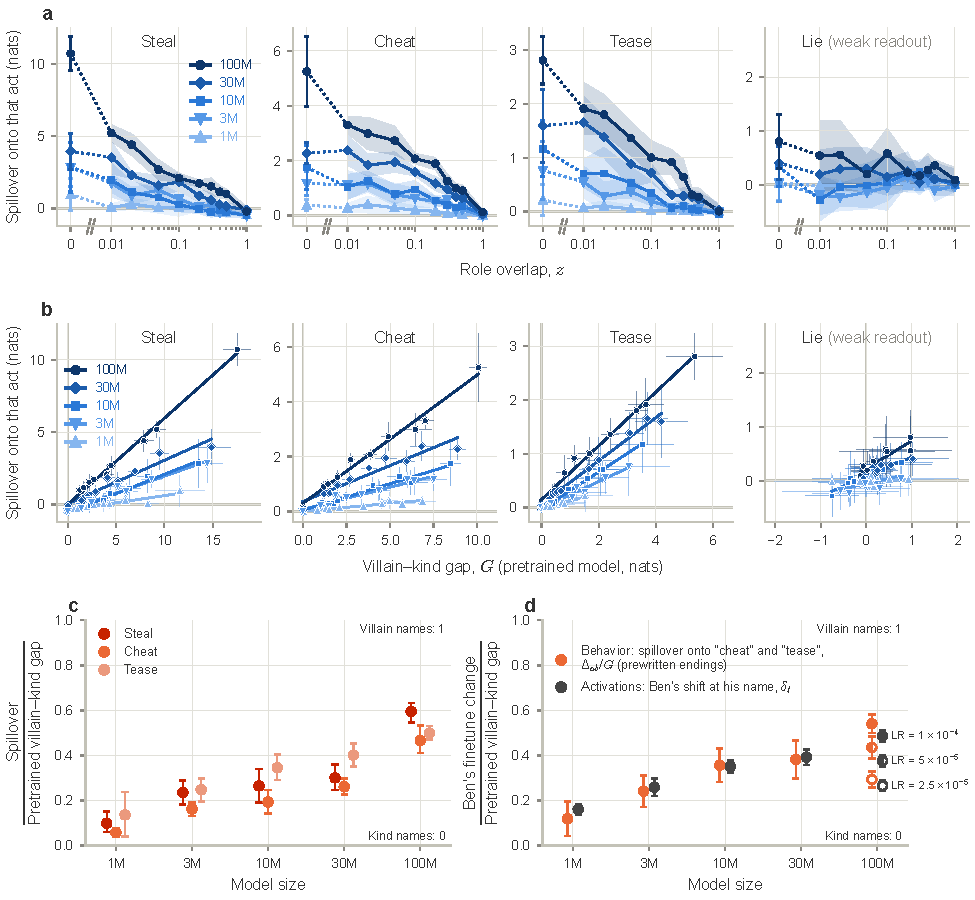
\includegraphics[width=\textwidth]{fig5_graded_and_size.pdf}
  \caption{
    \textbf{Spillover vs. corpus and model size.}
    All corpora in the ``villain/kind names'' family.
    Spillover averaged over 16 prewritten items per act, as in \cref{fig:test}b.
    Bands and error bars: 95\% CI over 8 seeds.
    Peak finetune learning rate is $10^{-4}$ unless noted.
    \panel{a}
    Spillover onto each act, averaged over finetunes on the other acts, vs. role overlap $z$ ($z=0$: generalist villains, $z=1$: names are random, see \cref{fig:design}c) and model size.
    10 corpora per size, each point the mean over 8 seeds.
    Log axis with break for $z=0$, as in \cref{fig:persona}a.
    \panel{b}
    Same data as \textbf{a}, replotted against the corresponding villain-kind gaps of the pretrained models.
    Lines: linear fit for each model size, with intercept, over its 10 corpora.
    \panel{c}
    (exploratory) Ratio of spillover to pretrained villain-kind gap vs. model size. Values are the slopes of the fits in \textbf{b} (excluding ``lie'').
    Intervals: 95\% from resampling the seeds (2,000 resamples).
    \panel{d} (exploratory)
    Normalized change in Ben's behavior and activations from finetuning ``Ben steals,'' for $z=0$, vs. model size.
    For behavior, we average the spillover onto ``cheat'' and ``tease,'' normalized to the pretrained villain-kind gap (see \cref{fig:persona,fig:test}).
    For activations, we compare the activations of the first \texttt{\textvisiblespace Ben} token in each prewritten item (64 items: 16 for each act) between the ``Ben steals'' finetune and the neutral finetune.
    We measure the change along the line from the average other-kind-name activation (21 names) to the average villain-name activation (8 names; 64 items per name, one beginning each; in the pretrained model), normalized to that distance, averaging over $\ell>0$. See text.
    LR: peak finetune learning rate.
    8 seeds at each learning rate.
  }
  \label{fig:graded}
\end{figure}
